The correctness of the algorithm follows by induction over the construction:
If the correct co-routine stops in the end state for all possible
constructions of the Thompson construction under the assumption that simpler
automata do the same, it follows that no matter how complex the automata get,
the algorithm will have the correct output.

The proof will be in three steps:
\begin{description}
  \item[Foundation] Firstly we will show that a simple path
    will get the correct indices, i.e. that the indexing of the capture works correctly.
  \item[Induction] Secondly we will show that an automaton constructed from
    correct sub-automata is correct.
  \item[Exhaustion] Thirdly and lastly we will show that every construction
    of the automata satisfies the induction property and thus that every
    automaton created by the modified Thompson construction is executed correctly.
\end{description}

But first we need to formalize the concept of a correct match and of greediness.

\begin{defn}
  A NFA $A$ is \emph{well-formed} if there is a regular expression $r$ that
  will be compiled to $A$ via the execution of algorithm~\ref{TODO(modified thompson}.

  Specifically this means that opening and closing of groups happens in
  correct order and that there is no path avoiding the closing of the group
  in case the opening is passed. Further a well-formed automaton can be
  deconstructed into subautomata corresponding to the Thompson construction.
\end{defn}

\begin{defn}
  A NFA $A$ is a \emph{chain} of subautomatons
  $A_1\rightarrow A_2 \rightarrow \dots \rightarrow A_m$ if it is well-formed
  and the picture
  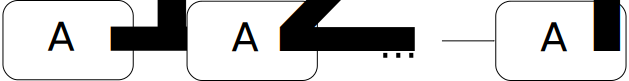
\includegraphics[width=0.8\linewidth]{graphs/chain}

  holds, i.e. the NFA $A_i$ appear in order and there are only 
  $\varepsilon$-transitions forward.
\end{defn}

\begin{defn}
  \includegraphics[width=0.8\linewidth]{graphs/backward}

  An NFA like the one above is called \emph{greedy} if the forward
  transition is down-prioritized:

  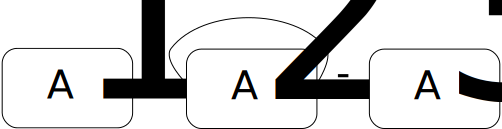
\includegraphics[width=0.8\linewidth]{graphs/backward-greedy}

  It is called non-greedy if the backward transition is down-prioritized:

  \includegraphics[width=0.8\linewidth]{graphs/backward-non}
\end{defn}

\begin{defn}
  A \emph{correct DFA state} is a list of coroutines that is ordered in the 
  half-order $<$ such that:
  \begin{description}
    \item[Simple transition $a\xrightarrow^{x} b$] $a<b$ if $x$ matches the 
      string.
    \item[Chain $A\rightarrow B$] $a_{begin}<a_{end}<b_{begin}<b_{end}$
    \item[Greedy loop $A*$] $a_{begin} < a_{end} < a_{middle}$
    \item[Non-greedy loop $A*?$] $a_{begin} < a_{middle} < a_{end}$
    \item[Alternation $A|B$] $b_{begin} < a_{begin}$ and 
      $b_{end} < a_{end}$ iff $A$ matches the string.
  \end{description}
\end{defn}

\begin{lemma}
  For a correct DFA state and a character $s_0$ the algorithm~\ref{TODO one 
  step} will produce a correct DFA state.
\end{lemma}

\begin{defn}
  A \emph{correct match} of a well-formed NFA $A$ on a string 
  $s=\"s_1s_2\dots s_n\"$ is defined inductively:

  \begin{description}
    \item[Simple transition $a\xrightarrow^{x} b$] if a coroutine ends in $b$, 
      it will have the memory of the coroutine in $a$ and the only character 
      read will be $x$.
    \item[Chain $A\rightarrow B$] the coroutine at the end of $B$ is the one 
      that first took the longest correct match in $A$ and then a correct 
      match in $B$.
    \item[(Non-)greedy loop] the coroutine at the end state is the one that 
      captured the most (least) letters in the automaton before exiting.
    \item[Alternation $A|B$] the coroutine at the end is the one through $A$ 
      if there exists a correct match and the one through $B$ otherwise (if any).
  \end{description}
\end{defn}

\begin{lemma}
  A correct DFA state contains the correct match.
\end{lemma}
\begin{proof}
  TODO
\end{proof}

\begin{lemma}\label{foundat}
  Algorithm~\ref{TODO} matches the empty string correctly.
\end{lemma}
\begin{proof}
  This corresponds to the epsilon transitions working correctly and is itself 
  best understood as a recursive property.

  \begin{description}
    \item[Simple transition] There is no correct match and the algorithm 
      will fail because no transitions are available.
    \item[Chain $A\rightarrow B$] Assuming that the correct coroutine 
      finishes $A$, then that is the only entry to $B$. Since there is no 
      character to capture, length of matches don't matter. Assuming that the 
      correct coroutine ends $B$, the algorithm will return the correct match.
    \item[(Non-)greedy loop] Again the length of the iteration doesn't 
      matter. Since visited states are not examined again, no endless loops 
      occur and thus no actual loop is taken. The correctness follows from 
      the correctness of the subautomaton.
    \item[Alternation $A|B$] If $A$ matches the empty string, then this 
      coroutines wins since $A$'s start state is put on the high priority stack.
      If $A$ fails, then the high priority stack must be empty (notice that 
      we understand the alternation to be the outmost part of the NFA) and 
      the start state of $B$ is considered.
  \end{description}
\end{proof}

\begin{lemma}\label{induc}
  Given that the NFA executed algorithm~\ref{TODO} on $s=s_1\dots s_{n-1}$ 
  then executing algorithm~\ref{TODO one step} on $s_{n}$ will give a correct 
  match for $ss_{n}$.
\end{lemma}
\begin{proof}
  This induction step proves that after a single step the coroutines are in 
  proper order.
\end{proof}

\begin{thm}
  Algorithm~\ref{TODO} matches all strings correctly.
\end{thm}
\begin{proof} This follows directly from lemma~\ref{foundat} and 
  lemma~\ref{induc} by induction.
\end{proof}
